\documentclass[crop]{standalone}

\usepackage{amsmath}

\usepackage[dvipsnames]{xcolor}
\usepackage{tikz}

\usetikzlibrary{shapes,decorations,arrows,calc,arrows.meta,fit,positioning}
\tikzset{
    -latex,
    node distance =1 cm and 1 cm,
    inner sep =0.15cm,
    semithick,
    O/.style ={rounded rectangle, draw, minimum width = 0.7 cm},
    U/.style ={rounded rectangle, draw, minimum width = 0.7 cm, dashed},
    fontscale/.style = {font=\huge}
}

\begin{document}


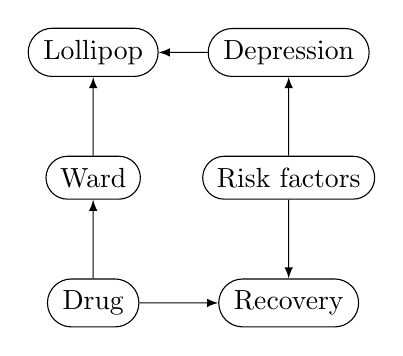
\begin{tikzpicture}
  \node[O] (x) at (0,0) {Drug};
  \node[O] (y) [right=of x] {Recovery};
  \node[O] (w) [above=of x] {Ward};
  \node[O] (l) [above=of w] {Lollipop};
  \node[O] (rf) [above=of y] {Risk factors};
  \node[O] (d) [above=of rf] {Depression};
  \path (x) edge (y);
  \path (x) edge (w);
  \path (w) edge (l);
  \path (rf) edge (y);
  \path (rf) edge (d);
  \path (d) edge (l);

\end{tikzpicture}


\end{document}
